\chapter{Semantische Suche}
\section{Definition}
Die semantische Suche beschreibt das Durchstöbern von Informationssammlung auf Grundlage von Beziehungen, Kenntnissen und Bedeutung über den jeweils gesuchten Begriff. Im Gegensatz zur Keyword-Suche, die lediglich Schlagwörter entdecken kann, wenn diese buchstäblich vorhanden sind, berücksichtigt die semantische Suche beispielsweise Synonyme oder andere Kontexte, die zu dem Suchbegriff passen.\newline
Grundlage der semantischen Suche ist oftmals eine Ontologie, die es ermöglicht, einen Überblick über Beziehung und Bedeutung eines Begriffs einem bestimmten Kontext zu erfassen. Mit Hilfe der Metadaten, die sich aus einer Ontologie ergeben kann das Finden von Informationen auf verschiedene Weise unterstützt werden.\newline

\begin{itemize}
    \item Query String Refinement\newline
          Query String Refinement beschreibt das präzisieren einer Suchanfrage durch das erweitern um Begriffe. Mit Hilfe einer zugrundeliegenden Ontologie kann durch das hinzufügen von Begriffen bei der Suche das Ergebnis thematisch eingeschränkt werden, da innerhalb der Ontologie möglicherweise z.B. mehrfach die Ausprägung Golf besteht, aber durch das Erweitern um \"Pkw\" keine weiteren Beziehungen im Bereich des Sports gefunden werden können und somit nur noch die gewünschten Ergebnisse vorhanden sind. 
    \item Inference\newline
          Bei Inference geht es um die implizierten Verknüpfungen zwischen Begriffen, die entstehen, wenn Knoten innerhalb der Ontologie über Beziehungen z.B. transitiv verbunden sind. Beispielsweise gehört eine Instanz explizit einer Unterklasse an, wird sie implizit auch der Oberklasse angehören. Ist beispielsweise \"Max\" teil der Unterklasse \"Vater\" der Klasse \"Mann\", lässt sich schließen, das \"Max\" auch der Klasse \"Mann\" angehört.
    \item Cross Referencing\newline
          Unter Cross Referencing wird das herstellen von Querverweisen un Assoziationen verstanden. Ähnlich wie bei Inference werden hier Rückschlüsse über die Zugehörigkeit anderer Klassen zum Suchbegriff gezogen. So ist zum Beispiel bei der Suche nach \"Hochschule Darmstadt\" eine mögliche Assoziation \"Technische Universität Darmstadt\", da es sich bei beidem Einrichtungen um eine akademische Bildungsstätte innerhalb der selben Stadt handelt. Entsprechend wären die Ergebnisse vermutlich über \"Ort\" oder \"Bildung\" Klassen veknüpft.
    \item Explorative Suche\newline
          Die explorative Suche orientiert sich weniger an üblichen technischen Sucherergebnissen wie eine Volltextsuche, sondern am "stöbern". Die Idee ist, dass man durch Angabe eines ungefähren Themas bereits Ergebnisse bieten kann, die in die ungefähre Richtung des gewünschten Ergebnissen gehen, aber ohne dass man wissen muss welche Begriffe man genau sucht. Durch Assoziationen und Implikationen durch die Vielzahl der Klassen innerhalb der Ontologien können dann weitere Vorschläge gegeben werden, durch die man sich durchstöbern kann und die einem mehr Informationen geben. Das ist ähnlich der Art, wie man sich auf Video oder Streamingplattformen Vorschläge nach bsow. Genre geben lassen kann, durch die man durchstöbern kann bis man schließlich den gewünschten Film erhält.
\end{itemize}
\cite{Sack.2010}
\section{Umsetzung}
Um zu überprüfen, ob und wie die semantische Suche in der Testfallontologie von Access Manager verwendet werden kann, werden die 4 Arten der Information Retrieval Unterstützung schrittweise versucht anzuwenden, um bestimmte Testfälle zu finden.
Angenommen die Ontologie aus dem vorherigen Kapitel sei nahezu vollständig umfassend und auch ausreichen mit Präzisierungen bezüglich Namen gefüllt. Jetzt will man einen Testfall suchen und schauen, was alles damit zusammenhängt.\\

Query String Refinement\newline
Ich suche alle Testfälle mit schreibrechten, damit bekommen ich wahrscheinlich ca. 50 Prozent aller Testfälle als Ergebnis. Da in der Ontologie jedoch noch Ordner und Domänen verlinkt sind, kann ich durch Angabe einer Domäne für den User und den Server präzisieren, dass ich nur die Tests erhalten möchte, die auf einer bestimmten Domain laufen.\\

Inference\newline
Wenn ich durch eine Suche alle Server erhalte, ist durch die Verknüpfung mit einem DomainMode klar, dass der Server Singledomain, Multidomain oder Multidomain Optimized ist. Erweitert man die Ontologie um die Regel, dass nur ein DomainMode zutreffen kann und sie sich gegenseitig ausschließen, ist klar, welche DomainMode Vorschriften welchen Server betreffen, und somit auch welche Testfälle.\\

Cross Referencing \newline
Assoziationen innerhalb der Testfälle lassen sich insofern als Suchergebnis liefern, dass die Testfälle mit verschiedenen Domains wahrscheinlich nicht zu den positiven SingleDomain Tests gehört. Falls man die Ontologie nun also noch so erweitert, das Postivtests („Dieser Fall soll passieren und läuft erfolgreich) und Negativtests („Dieser Fall darf so nicht passieren und muss fehlschlagen oder abgefangen werden“) unterteilt sind, lassen sich bei der Suche innerhalb der Berechtigungsvergabetests die Singledomain Tests aussschließen, da hier ja keine Fremddomain Nutzer auf einem Server berechtigt werden können. \newline
Hier lässt sich der Nutzen noch besser an einem größeren Beispiel erkennen. Nehmen wir an in einem anderen Team wurde eine weitere Ontologie erstellt, diesmal mit Fokus auf einen anderen Bereich der Tests, nämlich dem Profilmanagement. Diese Ontologien werden nun gemerged.\\

\begin{center}
    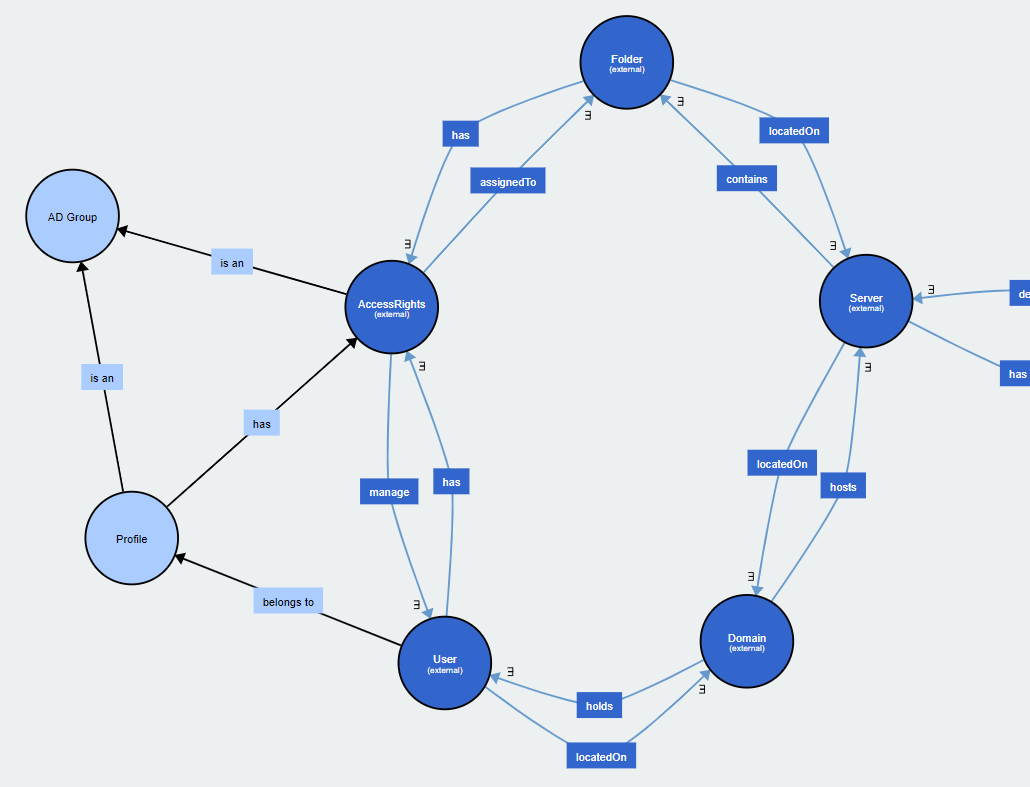
\includegraphics[width=1\textwidth]{Thesis/Images/OntologyProfiles.png}
\end{center}

Die Ontologie wurde nun um einen Aspekt der Profiltestfälle erweitert. Dadurch lassen sich einfach Assoziationen zwischen den Beiden Testarten ziehen. Profiltests und Usertests sind zum Beispiel beides Berechtigungsmanagement tests. Ebenso betreffen beide das Active Directory (Zugriffsverwaltung von Windwos). Dadurch können „ähnliche“ Tests bei einer Suche berücksichtigt werden.\\

Explorative Suche\newline
„Recommended“ testfälle wirken vielleicht erstmal etwas komisch, könnten aber durchaus einen praktischen Nutzen entwickeln. Wenn ich als neuer Verantwortlicher für Produktqualität mir einen Überblick verschaffen möchte, welche Testfälle es so gibt, oder was allgemein getestet wird, kann ich mich von den implizierten Verbindungen zwischen Tests leiten lassen. So sehe ich dann nach und nach, welche Domainmodes es gibt, wie diese Berücksichtigt werden usw. Sinnvoller wäre diese Form wohl bei mehreren Features, also nicht nur einem konkreten Testfallbereich, sondern einer Vielzahl an Features und Testfällen, die abgesehen vom Produkt, zunächst nicht viel zusammenhänge zu haben scheinen. Nach und nach kann man sich aber durch die AD-Tests, Job-Tests oder UI Tests leiten lassen. 

